\begin{frame}{\footnotesize [Υ3] Κατανομές μέσων σφαλμάτων εκτίμησης στάσης ανά μέθοδο ανάδρασης υπόθεσης \texttt{sm2} $[(\text{m}^2+\text{rad}^2)^{1/2}]$}

  \noindent\makebox[0.65\linewidth][c]{%
  \begin{minipage}{0.75\linewidth}

    \begin{figure}
      % GNUPLOT: LaTeX picture with Postscript
\begingroup
  \makeatletter
  \providecommand\color[2][]{%
    \GenericError{(gnuplot) \space\space\space\@spaces}{%
      Package color not loaded in conjunction with
      terminal option `colourtext'%
    }{See the gnuplot documentation for explanation.%
    }{Either use 'blacktext' in gnuplot or load the package
      color.sty in LaTeX.}%
    \renewcommand\color[2][]{}%
  }%
  \providecommand\includegraphics[2][]{%
    \GenericError{(gnuplot) \space\space\space\@spaces}{%
      Package graphicx or graphics not loaded%
    }{See the gnuplot documentation for explanation.%
    }{The gnuplot epslatex terminal needs graphicx.sty or graphics.sty.}%
    \renewcommand\includegraphics[2][]{}%
  }%
  \providecommand\rotatebox[2]{#2}%
  \@ifundefined{ifGPcolor}{%
    \newif\ifGPcolor
    \GPcolorfalse
  }{}%
  \@ifundefined{ifGPblacktext}{%
    \newif\ifGPblacktext
    \GPblacktexttrue
  }{}%
  % define a \g@addto@macro without @ in the name:
  \let\gplgaddtomacro\g@addto@macro
  % define empty templates for all commands taking text:
  \gdef\gplfronttext{}%
  \gdef\gplfronttext{}%
  \makeatother
  \ifGPblacktext
    % no textcolor at all
    \def\colorrgb#1{}%
    \def\colorgray#1{}%
  \else
    % gray or color?
    \ifGPcolor
      \def\colorrgb#1{\color[rgb]{#1}}%
      \def\colorgray#1{\color[gray]{#1}}%
      \expandafter\def\csname LTw\endcsname{\color{white}}%
      \expandafter\def\csname LTb\endcsname{\color{black}}%
      \expandafter\def\csname LTa\endcsname{\color{black}}%
      \expandafter\def\csname LT0\endcsname{\color[rgb]{1,0,0}}%
      \expandafter\def\csname LT1\endcsname{\color[rgb]{0,1,0}}%
      \expandafter\def\csname LT2\endcsname{\color[rgb]{0,0,1}}%
      \expandafter\def\csname LT3\endcsname{\color[rgb]{1,0,1}}%
      \expandafter\def\csname LT4\endcsname{\color[rgb]{0,1,1}}%
      \expandafter\def\csname LT5\endcsname{\color[rgb]{1,1,0}}%
      \expandafter\def\csname LT6\endcsname{\color[rgb]{0,0,0}}%
      \expandafter\def\csname LT7\endcsname{\color[rgb]{1,0.3,0}}%
      \expandafter\def\csname LT8\endcsname{\color[rgb]{0.5,0.5,0.5}}%
    \else
      % gray
      \def\colorrgb#1{\color{black}}%
      \def\colorgray#1{\color[gray]{#1}}%
      \expandafter\def\csname LTw\endcsname{\color{white}}%
      \expandafter\def\csname LTb\endcsname{\color{black}}%
      \expandafter\def\csname LTa\endcsname{\color{black}}%
      \expandafter\def\csname LT0\endcsname{\color{black}}%
      \expandafter\def\csname LT1\endcsname{\color{black}}%
      \expandafter\def\csname LT2\endcsname{\color{black}}%
      \expandafter\def\csname LT3\endcsname{\color{black}}%
      \expandafter\def\csname LT4\endcsname{\color{black}}%
      \expandafter\def\csname LT5\endcsname{\color{black}}%
      \expandafter\def\csname LT6\endcsname{\color{black}}%
      \expandafter\def\csname LT7\endcsname{\color{black}}%
      \expandafter\def\csname LT8\endcsname{\color{black}}%
    \fi
  \fi
  \setlength{\unitlength}{0.02500bp}%
  \begin{picture}(10000.00,4000.00)%
    \gplgaddtomacro\gplfronttext{%
      \colorrgb{0.00,0.00,0.00}%
      \put(1168,440){\makebox(0,0)[r]{\strut{} \scriptsize $0.0$}}%
      \colorrgb{0.00,0.00,0.00}%
      \put(1168,983){\makebox(0,0)[r]{\strut{} \scriptsize $0.01$}}%
      \colorrgb{0.00,0.00,0.00}%
      \put(1168,1526){\makebox(0,0)[r]{\strut{}\scriptsize $0.02$}}%
      \colorrgb{0.00,0.00,0.00}%
      \put(1168,2070){\makebox(0,0)[r]{\strut{}\scriptsize $0.03$}}%
      \colorrgb{0.00,0.00,0.00}%
      \put(1168,2613){\makebox(0,0)[r]{\strut{}\scriptsize $0.04$}}%
      \colorrgb{0.00,0.00,0.00}%
      \put(1168,3156){\makebox(0,0)[r]{\strut{}\scriptsize $0.05$}}%
      \colorrgb{0.00,0.00,0.00}%
      \put(1168,3699){\makebox(0,0)[r]{\strut{}\scriptsize $0.06$}}%
      \colorrgb{0.00,0.00,0.00}%
      \put(1625,220){\makebox(0,0){\strut{}\tiny {open}}}%
      \colorrgb{0.00,0.00,0.00}%
      \put(2493,220){\makebox(0,0){\strut{}\tiny {soft-$1$}}}%
      \colorrgb{0.00,0.00,0.00}%
      \put(3361,220){\makebox(0,0){\strut{}\tiny {soft-$50$}}}%
      \colorrgb{0.00,0.00,0.00}%
      \put(4229,220){\makebox(0,0){\strut{}\tiny {hard}}}%
      \colorrgb{0.00,0.00,0.00}%
      %\put(398,2069){\rotatebox{90}{\makebox(0,0){\strut{}$\overline{\|e\|_{2,i}}$, $i = \{1,2,\dots,N\}$}}}%
      \put(-98,2069){\rotatebox{90}{\makebox(0,0){\strut{}\footnotesize CORRIDOR}}}%
      %\colorrgb{0.00,0.00,0.00}%
      %\put(2927,-110){\makebox(0,0){\strut{}Μέθοδος ανάδρασης}}%
      %\colorrgb{0.00,0.00,0.00}%
      %\put(2927,4029){\makebox(0,0){\strut{}Κατανομή μέσων σφαλμάτων εκτίμησης στάσης ανά μέθοδο ανάδρασης}}%
    }%
    \gplgaddtomacro\gplfronttext{%
    }%
    \gplgaddtomacro\gplfronttext{%
      \colorrgb{0.00,0.00,0.00}%
      \put(5663,440){\makebox(0,0)[r]{\strut{}\scriptsize $0.011$}}%
      \colorrgb{0.00,0.00,0.00}%
      \put(5663,2070){\makebox(0,0)[r]{\strut{}\scriptsize $0.0115$}}%
      \colorrgb{0.00,0.00,0.00}%
      \put(5663,3699){\makebox(0,0)[r]{\strut{}\scriptsize $0.012$}}%
      \colorrgb{0.00,0.00,0.00}%
      \put(6120,220){\makebox(0,0){\strut{}\tiny {open}}}%
      \colorrgb{0.00,0.00,0.00}%
      \put(6988,220){\makebox(0,0){\strut{}\tiny {soft-$1$}}}%
      \colorrgb{0.00,0.00,0.00}%
      \put(7856,220){\makebox(0,0){\strut{}\tiny {soft-$50$}}}%
      \colorrgb{0.00,0.00,0.00}%
      \put(8724,220){\makebox(0,0){\strut{}\tiny {hard}}}%
      \colorrgb{0.00,0.00,0.00}%
      %\put(7422,-110){\makebox(0,0){\strut{}Μέθοδος ανάδρασης}}%
      %\colorrgb{0.00,0.00,0.00}%
      %\put(7422,4029){\makebox(0,0){\strut{}CORRIDOR pose errors per feedback method}}%
      \put(2927,4029){\makebox(0,0){\strut{}\scriptsize Πλήρης άποψη}}%
      \put(7422,4029){\makebox(0,0){\strut{}\scriptsize Εστιασμένη άποψη}}%
    }%
    \gplgaddtomacro\gplfronttext{%
    }%
    \put(0,0){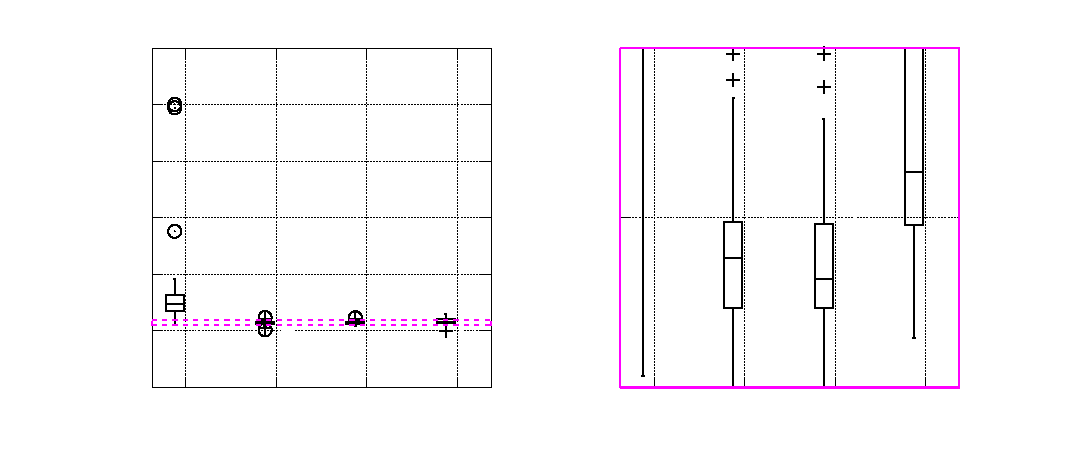
\includegraphics[scale=0.5]{./figures/slides/ch4/experiments/boxplots/corridor_mean_total_errors_per_feedback}}%
    \gplfronttext
  \end{picture}%
\endgroup

    \end{figure}
    \vspace{-0.8cm}
    \begin{figure}
      % GNUPLOT: LaTeX picture with Postscript
\begingroup
  \makeatletter
  \providecommand\color[2][]{%
    \GenericError{(gnuplot) \space\space\space\@spaces}{%
      Package color not loaded in conjunction with
      terminal option `colourtext'%
    }{See the gnuplot documentation for explanation.%
    }{Either use 'blacktext' in gnuplot or load the package
      color.sty in LaTeX.}%
    \renewcommand\color[2][]{}%
  }%
  \providecommand\includegraphics[2][]{%
    \GenericError{(gnuplot) \space\space\space\@spaces}{%
      Package graphicx or graphics not loaded%
    }{See the gnuplot documentation for explanation.%
    }{The gnuplot epslatex terminal needs graphicx.sty or graphics.sty.}%
    \renewcommand\includegraphics[2][]{}%
  }%
  \providecommand\rotatebox[2]{#2}%
  \@ifundefined{ifGPcolor}{%
    \newif\ifGPcolor
    \GPcolorfalse
  }{}%
  \@ifundefined{ifGPblacktext}{%
    \newif\ifGPblacktext
    \GPblacktexttrue
  }{}%
  % define a \g@addto@macro without @ in the name:
  \let\gplgaddtomacro\g@addto@macro
  % define empty templates for all commands taking text:
  \gdef\gplfronttext{}%
  \gdef\gplfronttext{}%
  \makeatother
  \ifGPblacktext
    % no textcolor at all
    \def\colorrgb#1{}%
    \def\colorgray#1{}%
  \else
    % gray or color?
    \ifGPcolor
      \def\colorrgb#1{\color[rgb]{#1}}%
      \def\colorgray#1{\color[gray]{#1}}%
      \expandafter\def\csname LTw\endcsname{\color{white}}%
      \expandafter\def\csname LTb\endcsname{\color{black}}%
      \expandafter\def\csname LTa\endcsname{\color{black}}%
      \expandafter\def\csname LT0\endcsname{\color[rgb]{1,0,0}}%
      \expandafter\def\csname LT1\endcsname{\color[rgb]{0,1,0}}%
      \expandafter\def\csname LT2\endcsname{\color[rgb]{0,0,1}}%
      \expandafter\def\csname LT3\endcsname{\color[rgb]{1,0,1}}%
      \expandafter\def\csname LT4\endcsname{\color[rgb]{0,1,1}}%
      \expandafter\def\csname LT5\endcsname{\color[rgb]{1,1,0}}%
      \expandafter\def\csname LT6\endcsname{\color[rgb]{0,0,0}}%
      \expandafter\def\csname LT7\endcsname{\color[rgb]{1,0.3,0}}%
      \expandafter\def\csname LT8\endcsname{\color[rgb]{0.5,0.5,0.5}}%
    \else
      % gray
      \def\colorrgb#1{\color{black}}%
      \def\colorgray#1{\color[gray]{#1}}%
      \expandafter\def\csname LTw\endcsname{\color{white}}%
      \expandafter\def\csname LTb\endcsname{\color{black}}%
      \expandafter\def\csname LTa\endcsname{\color{black}}%
      \expandafter\def\csname LT0\endcsname{\color{black}}%
      \expandafter\def\csname LT1\endcsname{\color{black}}%
      \expandafter\def\csname LT2\endcsname{\color{black}}%
      \expandafter\def\csname LT3\endcsname{\color{black}}%
      \expandafter\def\csname LT4\endcsname{\color{black}}%
      \expandafter\def\csname LT5\endcsname{\color{black}}%
      \expandafter\def\csname LT6\endcsname{\color{black}}%
      \expandafter\def\csname LT7\endcsname{\color{black}}%
      \expandafter\def\csname LT8\endcsname{\color{black}}%
    \fi
  \fi
  \setlength{\unitlength}{0.0500bp}%
  \begin{picture}(10000.00,4000.00)%
    \gplgaddtomacro\gplfronttext{%
      \colorrgb{0.00,0.00,0.00}%
      \put(1168,1081){\makebox(0,0)[r]{\strut{}$1.0$}}%
      \colorrgb{0.00,0.00,0.00}%
      \put(1168,1736){\makebox(0,0)[r]{\strut{}$2.0$}}%
      \colorrgb{0.00,0.00,0.00}%
      \put(1168,2390){\makebox(0,0)[r]{\strut{}$3.0$}}%
      \colorrgb{0.00,0.00,0.00}%
      \put(1168,3045){\makebox(0,0)[r]{\strut{}$4.0$}}%
      \colorrgb{0.00,0.00,0.00}%
      \put(1168,3699){\makebox(0,0)[r]{\strut{}$5.0$}}%
      \colorrgb{0.00,0.00,0.00}%
      \put(1625,220){\makebox(0,0){\strut{}open}}%
      \colorrgb{0.00,0.00,0.00}%
      \put(2493,220){\makebox(0,0){\strut{}soft-$1$}}%
      \colorrgb{0.00,0.00,0.00}%
      \put(3361,220){\makebox(0,0){\strut{}soft-$50$}}%
      \colorrgb{0.00,0.00,0.00}%
      \put(4229,220){\makebox(0,0){\strut{}hard}}%
      \colorrgb{0.00,0.00,0.00}%
      \put(530,2069){\rotatebox{90}{\makebox(0,0){\strut{}$\overline{\|e\|_{2,i}}$, $i = \{1,2,\dots,N\}$}}}%
      \colorrgb{0.00,0.00,0.00}%
      \put(2927,-110){\makebox(0,0){\strut{}Μέθοδος ανάδρασης}}%
      \colorrgb{0.00,0.00,0.00}%
      %\put(4627,4029){\makebox(0,0){\strut{}Κατανομή μέσων σφαλμάτων εκτίμησης στο περιβάλλον WAREHOUSE ανά μέθοδο ανάδρασης}}%
    }%
    \gplgaddtomacro\gplfronttext{%
    }%
    \gplgaddtomacro\gplfronttext{%
      \colorrgb{0.00,0.00,0.00}%
      \put(5663,579){\makebox(0,0)[r]{\strut{}$0.025$}}%
      \colorrgb{0.00,0.00,0.00}%
      \put(5663,1272){\makebox(0,0)[r]{\strut{}$0.035$}}%
      \colorrgb{0.00,0.00,0.00}%
      \put(5663,1965){\makebox(0,0)[r]{\strut{}$0.045$}}%
      \colorrgb{0.00,0.00,0.00}%
      \put(5663,2659){\makebox(0,0)[r]{\strut{}$0.055$}}%
      \colorrgb{0.00,0.00,0.00}%
      \put(5663,3352){\makebox(0,0)[r]{\strut{}$0.065$}}%
      \colorrgb{0.00,0.00,0.00}%
      \put(6120,220){\makebox(0,0){\strut{}open}}%
      \colorrgb{0.00,0.00,0.00}%
      \put(6988,220){\makebox(0,0){\strut{}soft-$1$}}%
      \colorrgb{0.00,0.00,0.00}%
      \put(7856,220){\makebox(0,0){\strut{}soft-$50$}}%
      \colorrgb{0.00,0.00,0.00}%
      \put(8724,220){\makebox(0,0){\strut{}hard}}%
      \colorrgb{0.00,0.00,0.00}%
      \put(7422,-110){\makebox(0,0){\strut{}Μέθοδος ανάδρασης}}%
      \colorrgb{0.00,0.00,0.00}%
      %\put(7422,4029){\makebox(0,0){\strut{}WAREHOUSE pose errors per feedback method}}%
    }%
    \gplgaddtomacro\gplfronttext{%
    }%
    \gplfronttext
    \put(0,0){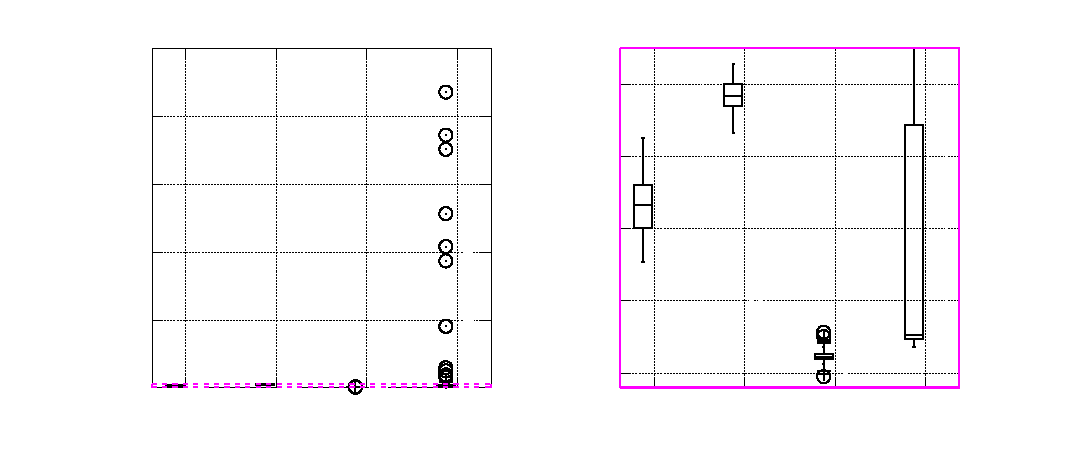
\includegraphics{./figures/parts/02/chapters/02/sections/04/warehouse_mean_total_errors_per_feedback}}%
    \gplfronttext
  \end{picture}%
\endgroup

    \end{figure}

  \end{minipage}
  }
  \noindent\makebox[0.3\linewidth][c]{%
    \begin{minipage}{0.3\linewidth}\tiny
      Πηγές:\\

      soft-1: \\
      G. Peng, W. Zheng, Z. Lu, J. Liao, L. Hu, G. Zhang, D. He, ``An improved AMCL algorithm based on laser scanning match in a complex and unstructured environment", \textit{Complexity}, 2018 \\

      soft-50: \\
      A. Filotheou, E. Tsardoulias, A. Dimitriou, A. Symeonidis, L. Petrou, ``Pose Selection and Feedback Methods in Tandem Combinations of Particle Filters with Scan-Matching for 2D Mobile Robot Localisation", \textit{Journal of Intelligent and Robotic Systems}, 2020 \\

      hard: \\
      G. Vasiljević, D. Miklić, I. Draganjac, Z. Kovačić, P. Lista, ``High-accuracy vehicle localization for autonomous warehousing", \textit{Robotics and Computer-Integrated Manufacturing}, 2016
    \end{minipage}
  }

\note{\footnotesize
και σε αυτή τη διαφάνεια βλέπουμε τα μέσα σφάλματα ανά μέθοδο
ανάδρασης. Εδώ με open συμβολίζουμε την open-loop κατάσταση, δηλαδή και πάλι
την ονομαστική κατάσταση του φίλτρου, με soft-1 τη διαμόρφωση όπου το
αποτέλεσμα του sm2 εισάγεται στον πληθυσμό του φίλτρου με τη μορφή ενός μόνο
σωματιδίου, με soft-50 τη διαμόρφωση όπου το αποτέλεσμα του sm2 εισάγεται στον
πληθυσμό με τη μορφή τόσων σωματιδίων όσών να αποτελούν το 50% του τελικού
πληθυσμού, και hard τη διαμόρφωση όπου το φίλτρο αρχικοποιείται εκ του μηδενός
γύρω από το αποτέλεσμα του sm2. Εδώ βλέπουμε πως γενικά η μέθοδος που εισάγαμε
εμφανίζει κατά μέσο όρο τα μικρότερα σφάλματα, και πως είναι πιο ανθεκτική από
τη μέθοδο hard.}


\end{frame}
